\chapter{Zweite Methode} \label{cha:ZweiteMethode}

In diesem Kapitel werden die erste Erfahrung beschrieben. Zuerst läuft die Vorstellung des DaVid-Systems. Die Systemmodell und Arbeitsprinzip des Systems werden in anschließenden Abschnitt erläutert. Schließlich folgt die mögliche Anwendungsgebiete des Systems.

Nicht vergessen, dass Überschriften nicht aufeinander folgen dürfen\ldots

\section{Allgemeine Struktur}


\section{Binariesierung}

\textbf{Grundlegende globale Schwelle Methode}

Wenn die Histogrammspitzen und -täler des Bildes offensichtlich sind und Doppelpeaks aufweisen, ist die Wirkung dieserMethode besser. Es basiert auf der visuellen Überprüfung des Histogramms und der Schwellenwert wird durch eine iterative Methode erhalten. Die grundlegende Algorithmus ist wie folgt:

1. Wählen eine Paramenter t und einen anfänglichen Schwellenwert $ T_{0} $ aus, wobei der Durchschnitt der maximalen Grauwerte $ l_{max} $ und minimalen Grauwerte  $ l_{max} $ verwendet wird. $ T_{0} = (l_{max}+l_{max})/2 $

2. Segmentieren das Bild mit dem Schwellenwert $ T_{0} $. Dann das Bild besteht aus zwei Teilen: $ G_{1} $ besteht aus die Pixeln mit deren Grauwert größer als $ T_{0} $ und dargegen $ G_{2} $ deren Grauwert kleiner oder gleich als $ T_{0} $.

3. Berechnen den durchschnittlichen Grauwert aller Pixeln in $ u_{1} $ und $ u_{2} $ und den neue Schwellenwert $ T_{1} = (u_{1}+u_{2})/2 $.

4. Falls $ |T_{0} - T_{1}| < t $, dann nehmen $ T_{1} $ als optimalen Schwellenwert. Andernfalls weisen $ T_{1} $ zu $ T_{0} $und wiederholen die Schritte $ 2\sim4 $, bis der optimale Schwellenwert erhalten ist.

\textbf{Grundlegende adaptive Schwellenwert Binarisierungsmethode}

Ein Bildgebungsfaktor ungleichmäßiger Helligkeit bewirkt, dass ein Histogramm, das ansonsten für eine effiziente Segmentierung geeignet wäre, ein Histogramm wird, das nicht effektiv mit einem einzigen globalen Schwellenwert segmentiert werden kann.

Ein Verfahren zur Verarbeitung besteht darin, das Bild weiter in Unterbilder zu unterteilen, um unterschiedliche Unterbilder mit unterschiedlichen Schwellenwerten zu segmentieren. Diese Methode wird als grundlegende adaptive Schwellenwert-Binarisierungsmethode bezeichnet. Das Hauptproblem bei diesem Ansatz besteht darin, das Bild zu unterteilen und den Schwellenwert für das resultierende Teilbild abzuschätzen. Da die Schwelle für jedes Pixel von dem Pixel in der Untergruppe abhängt, die Position im Bild, also solche Schwellen sind adaptiv. 

Ein Verfahren zum Unterteilen von Unterbildern wird für das Bild übernommen. Hier werden drei Arten von Unterteilungsverfahren ausgewählt, und Unterbildermit einer Größe von $ 32\times32,4 \times4,16\times16 $ Pixelwerden jeweils geteilt, und die durchschnittliche Graustufe der Unterbilder wird Sals ein Schwellenwert für die Binärisierung ausgewählt.


\textbf{OTSU adaptive Schwelle Methode}

OTSU\cite{Ostu}, auch bekannt als die maximale Interklassenvarianz, wurde 1979 vom japanischen Gelehrten Otsu vorgeschlagen und ist eine adaptive Schwellenwertbestimmungsmethode, die auch als Otsu bekannt ist.

Die Grundidee des Otsu-Algorithmus ist: Verwenden das Histogramm des Bildes, gemäß der Varianz zwischen dem Vordergrund und dem Hintergrund, um den optimalen Schwellenwert dynamisch zu bestimmen. Setze die Anzahl der Pixeln in einen Bilden ist N, die Graustufe ist $ L(0,1,...,L-1) $. Die Anzahl der Pixeln mit dem Grauswert i ist $ n_{i} $, dann die Wahrscheinlichkeit von i läuft $ P_{i} = \frac{n_{i}}{N} $. Für das Bild stellt das T die Segmentierungsschwellenwert zwischen Vordergrund und des Hintergrund dar. Vordergrund entsprecht die Grauswerte von 0 zu $ T-1 $, dagegen Hintergrund die Grauswerte von T zu $ L -1 $.

Die Wahrscheinlichkeit der Vordergrundgebiet W0 und der durchschnittliche Grauwert U0 sind

\begin{equation}
  w_{0} = \sum_{i=0}^{T-1} p_{i},\quad u_{0} = \sum_{i=0}^{T-1} ip_{i}/w_{0}
\end{equation}

dagegen die Wahrscheinlichkeit der Hintergrundpunkte W1 und der durchschnittliche Grauwert U1 sind

\begin{equation}
  w_{1} = \sum_{i=T}^{L-1} p_{i} = 1-w_{0},\quad u_{1} = \sum_{i=T}^{L-1} ip_{i}/w_{1}
\end{equation}

Dann das gesamte durchschnittliche Grauwert des Bildes ist

\begin{equation}
• u = w_{0}u_{0} + w_{1}u_{1}
\end{equation}

Die Infra-Klassen-Varianz ist definiert als

\begin{equation}
•\sigma^2 = w_{0}(u_{0} - u)^2 + w_{1}(u_{1} - u)^2 = w_{0}w_{1}(u_{0} - u_{1})^2
\end{equation}

Nehmen Schwellenwert T von 0 zu $ L-1 $. Wenn $ sigma^2 $ Maximum ist, wählen der entsprechende T als der optimale Schwellenwert aus.

Die Ostu-Methode verwendet Grauswert Histogramm zur Bestimmen des Schwellenwerts. Es ist eine automatisch non-parametrische Schwellenauswahlmethode. Diese Methode ist einfach zu berechnen, und wird nicht von der Kontrast- und Helligkeitsänderung unter bestimmten Bedingungen beeinflusst und kann das Objekt zufriedenstellend vom Hintergrundbereich trennen.

















\section{Morphologie}

Nach der Binarisierung kann das Bild zahlreiche Unvollkommenheiten erhalten. Insbesondere ist das Binärbild, die durch einfache Schwellenwert erteilt werden, durch Rauschen und Textur verzerrt. 
Die morphologische Bildverarbeitung verfolgt das Ziel, diese Unvollkommenheiten zu beseitigen, indem Form und Struktur des Objekts berücksichtigt werden.

Morphologische Operationen arbeiten auf der Grundlage der Mengenoperation und hängen von der relativen Ordnung des Pixelwerts ab. Diese Eigenschaft macht es besonders geeignet für die Verarbeitung von Binärbildern. Natürlich ist Mengenoperation gleichmäßig gültig für Graustufenbilder. Hier in dieser Arbeit wird es nur in binäre Bilder benutzt. Es erstellt ein neues Binärbild, bei dem das Pixel einen nicht-Null Wert hat, nur wenn der Operation an dieser Position im Eingabebild erfolgreich ist.

Die Eingabedaten für die mathematischen morphologischen Operationen sind zwei Bilder: das zu bearbeitende Bild A und ein Strukturelement B. B ist normalerweise eine kleine Pixelmatrix mit jeweils einem Wert von Null oder Eins. Einige Eigenschaft des Strukturelements werden wie folgend gelegt.

\begin{itemize}

\item Die Matrixdimensionen geben die Größe des Strukturelements an.
\item Das Muster, das aus Einsen und Nullen bestehen, gibt die Form des Strukturelements an.
\item Ein Ursprung des Strukturelements ist üblicherweise eines dessen Pixel, es verlassen sich auch außerhalb des Strukturelements liegen. 

\end{itemize}

Eine übliche Praxis besteht darin, dass ungerade Dimensionen der Pixelmatrix stellen und den Ursprung als das Zentrum der Matrix definieren. Einige grundlegende Strukturelement legt als folgen:

\begin{figure}[htb]
 \centering 
  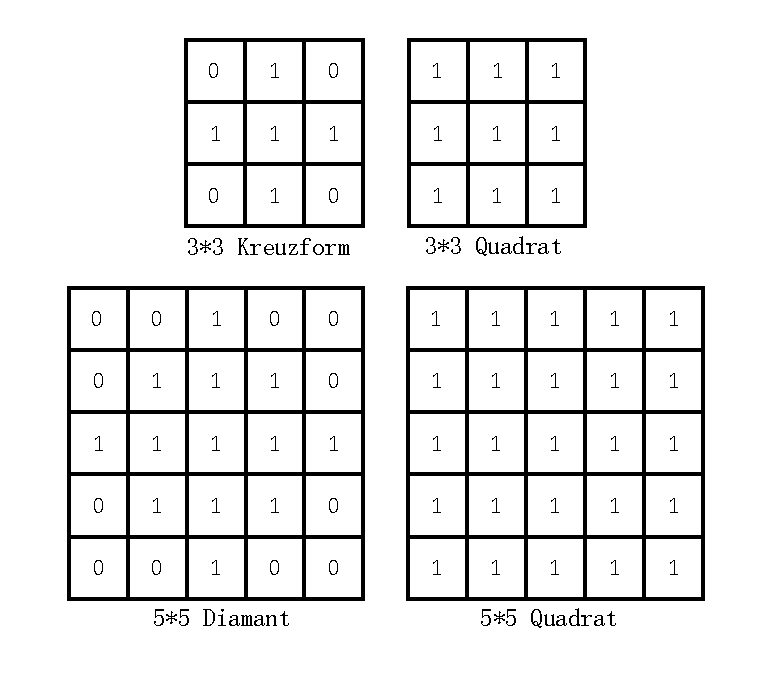
\includegraphics[keepaspectratio,width=0.6\textwidth]{images/4_ZweiteErfahrung/Morphological/strelement.pdf}
 \caption{Einige grundlegende Strukturelement}
 \label{fig:Strukturelement}
\end{figure} 

Als folgend werden zuerst die zwei grundlegende morphologischen Operatoren Erosion und Dilatation beschrieben. Anschließen vorstellen die darauf basierend Operationen, wie als Öffnung und Schließung bekannt sind.

\textbf{Dilatation}

Die Dilatation Operation bewirkt, dass das Objekt nach größer wächst. Das wächst Ausmaß hängt von der Art und Form des Strukturelements ab. Die Formel eine Dilatation wird darstellt als:

\begin{equation}
•A \oplus B =\lbrace z \mid \widehat{(B)_z} \cap A \ne \varnothing \rbrace  
\end{equation}

Hier $ \widehat{(B)_z} $ heißt Strukturelement B um seinen Ursprung reflektiert und um z verschoben. Die entsprechende Dilatation für das Bild A mit B ist die Menge aller Verschiebungen z, die $ \widehat{B} $ und A mindestens ein gemeinsames Element habe. Das Ergebnis der Dilatation läuft, die Pixeln um den Grenze des Objekts hinzufügen. Außerdem die Dilatation Operation wird im wesentlichen verwendet um die Löcher (fehlende Pixel) in einem kontinuierlichen Objekt zu füllen. Es beeinflusst die Intensität an diesem Bereich und kann als ein Unschärfe Effekt beobachtet werden, nämlich eine räumlichen Tiefpassfilter, die beim linearen Filtern des Bildes verwendet werden. Abbildung \ref{fig:Dilatation und Erosion} zeigt eine typische Dilatation Operation.

\begin{figure}[htb]
 \centering 
  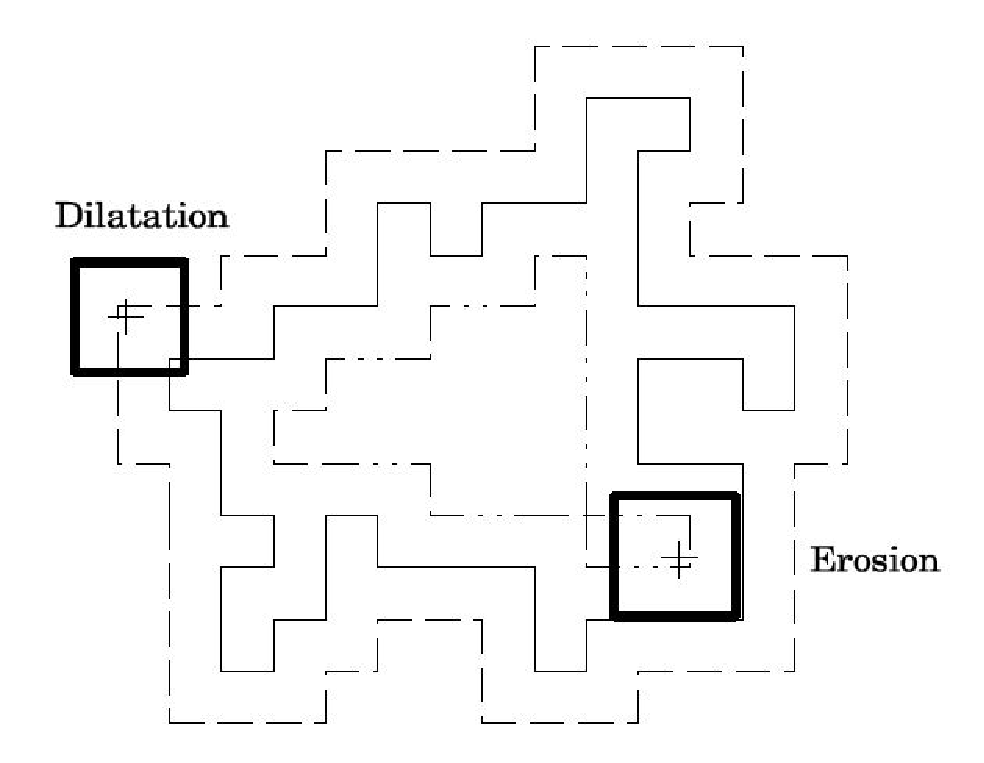
\includegraphics[keepaspectratio,width=0.8\textwidth]{images/4_ZweiteErfahrung/Morphological/DilatationundErosion.pdf}
 \caption{Dilatation und Erosion}
 \label{fig:Dilatation und Erosion}
\end{figure} 


\textbf{Erosion}

Der Operationseffekt eine Erosion ist genau ein Gegenteil von Dilatation. Die Erosion Operation bewirkt, dass das Objekt nach kleiner wechseln. Die Erosion eines Bildes A durch das Strukturelement B ist definiert als 

\begin{equation}
•A \ominus B =\lbrace z \mid (B)_z \subseteq A \rbrace  
\end{equation}

Hier die Erosion des Bilds A ist die Menge aller Punkte z mit derart, dass das Strukturelement B von verschieben wird, zu eine Teilmenge des Bildes A 	gehört. Diese Operation führt zu einem Verlust von Grenzpixeln des Objekts.

Die Erosion Operation entfernt solche Strukturen, die eine kleinere Größe als das strukturierende Element haben. Dann kann es verwenden wird, um die verrauschte "Verbindung" zwischen zwei Objekten zu entfernen. Da die unerwünschten Pixel entfernen werden, ist der Effekt als ein Schärfen des Objekts entsprechen. Als folgend in Abbildung \ref{fig:Dilatation und Erosion} zeigt eine typische Erosion Operation.


\textbf{Öffnung}

Die Öffnung Operation eines Bildes ist eine kombinatorische Operation von Erosion und Dilatation, d.h. zuerst nehmen eine Erosion Operation, danach eine Dilatation Operation. Praktisch werden Bild A durch beide Operationen mit dem gleichen Strukturelement B ausgeführt. Die Formel einer Öffnung Operation ist definiert als

\begin{equation}
•A \circ B =( A \ominus B )\oplus B  
\end{equation}

Die Grenze des geöffneten Objekts sind die Punkte, dass Strukturelement B die äußersten Punkte der Grenze von Objekt erreicht, wenn B innerhalb dieser Grenze entlangfahren. Feine strukturierte Details,
kleiner als das Strukturelement werden demnach beim Öffnung Operation entfernt, dünne Verbindungen zwischen größeren Teilen aufgelöst. Eine Öffnung Operation wird in Abbildung \ref{fig:oeffnungundschliessung} gezeigt.

\begin{figure}[htb]
 \centering 
  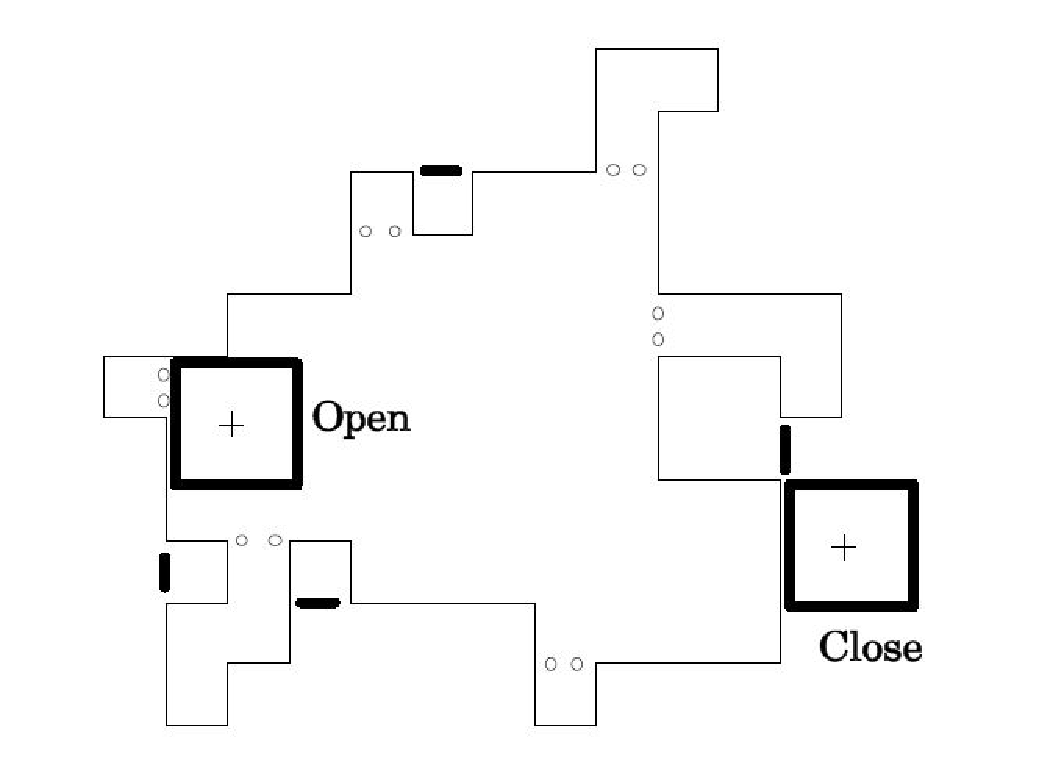
\includegraphics[keepaspectratio,width=0.8\textwidth]{images/4_ZweiteErfahrung/Morphological/oeffnungundschliessung.pdf}
 \caption{Einige grundlegende Strukturelement}
 \label{fig:oeffnungundschliessung}
\end{figure} 

\textbf{Schließung}

Gleichfalls mit Öffnung Operation ist die Schließung Operation auch eine kombinatorische Operation von Erosion und Dilatation. Der Unterschied dazwischen legt der Reihenfolge der Operation, d.h. hier zuerst eine Dilatation Operation, danach eine Erosion Operation mit dem gleichen Strukturelement. Das Schließung eines Bildes A durch das Strukturelement B ist definiert als

\begin{equation}
•A \bullet B =( A \oplus B )\ominus B  
\end{equation}

Die Grenze des geschlossenen Objekts sind die Punkte, dass Strukturelement B, die die äußersten Punkte der Grenze von Objekt erreichen, wenn B außerhalb dieser Grenze entlangfahren. Kleinere Risse, Lücken und feine Details werden dagegen aufgefüllt und mit den großen Teilen zusammengeschlossen. Abbildung \ref{fig:oeffnungundschliessung} zeigt eine Vorgang der Schließung Operation.


Öffnung und Schließung Operation besitzen die folgenden Eigenschaften:

\begin{itemize}

\item Öffnung und Schließung sind idempotent.
\item Die Öffnung Operation ist anti-extensiv. 
\item Die Schließung Operation ist extensiv.
\item Öffnung und Schließung sind dual bezüglich der Komplementierung.
\item Bezeichnet ein Bild als B-Öffnet, wenn es bezüglich gleicher Öffnung Operation unverändert bleibt. 
\item Bezeichnet ein Bild als B-Schließt, wenn es bezüglich gleicher Schließung Operation unverändert bleibt. 

\end{itemize}


\section{Canny detection}



\section{Hough detection}


